% figures/fd-decomposition.tex
\documentclass[11pt]{article}
\usepackage[margin=1.5cm]{geometry}
\usepackage{tikz}
\usetikzlibrary{positioning,arrows.meta}
\pagestyle{empty}
\begin{document}
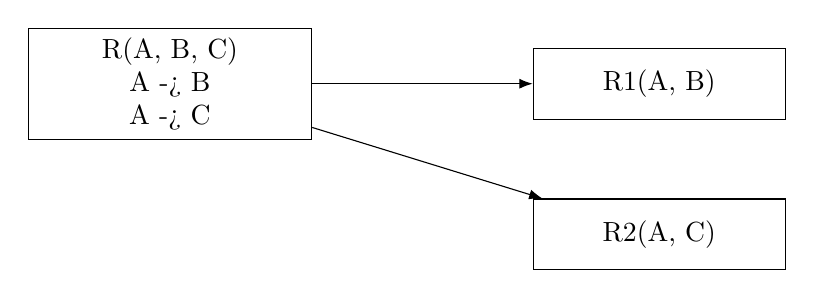
\begin{tikzpicture}[node distance=12mm, >=Latex]
  \node[draw, rectangle, minimum width=3.6cm, minimum height=1.0cm, align=center] (r) {R(A, B, C)\\A -> B\\A -> C};
  \node[draw, rectangle, minimum width=3.2cm, minimum height=0.9cm, right=28mm of r, align=center] (r1) {R1(A, B)};
  \node[draw, rectangle, minimum width=3.2cm, minimum height=0.9cm, below=10mm of r1, align=center] (r2) {R2(A, C)};
  \draw[->] (r) -- (r1);
  \draw[->] (r) -- (r2);
\end{tikzpicture}
\end{document}
